\chapter{Active Queue Management}

In Chapter \ref{cha:quality_metrics} we mentioned that some of the Internet applications are elastic in the sense that they make use of all the available bandwidth.
The interesting part is that these application don't know in advance how much bandwidht is available, which means that they have to find it out somehow.
In this chapter we describe how TCP congestion control and Active Queue Management (AQM) work together to throttle bandwidth hungry applications.

The interplay between TCP and AQM is critical to deliver satisfactory performance.
In 2009, mainstream media\footnote{E.g. www.nytimes.com/2009/09/03/technology/companies/03att.html} reported performance problems in AT\&T's wireless data network.
The alleged cause was the increase of data usage due to the popularity of IPhones.
The underlying reason seamed to be a poor buffer dimensioning\footnote{\url{http://blogs.broughturner.com/2009/10/is-att-wireless-data-congestion-selfinflicted.html}}.

\section{TCP congestion control}
We will introduce the working principles of TCP.
This is not meant to be an accurate description of TCP, just an overview of the concepts used for congestion control.
TCP is indeed very complex, heterogeneous (different in different OS), and continuously evolving.
An accurate description of TCP is beyond the scope of this course.

TCP is a flow-oriented transport (layer 4) protocol that is used by the elastic applications in Internet.
This includes most of the applications, such as web browsing, email and file transfer.
Take the example of a large file transfer using FTP, which involves the transmission of a large amount of data.
TCP doesn't know how much bandwidth is available, so it will start transmitting two MSS worth of data.
This is the initial value of the contention window (CW) which is the maximum amount of in-flight unacknowledged data is permitted.
The CW is increased in one MSS for each received acknowledgement.
This process is called the slow start phase of TCP.
Even though it starts slow, the truth is that it is growing exponentially and, at some point, the transmitting rate will exceed the available capacity and a packet will be dropped.

When TCP detects that a single packet has been dropped (signaled by a duplicate ack), it halves its congestion window and starts increasing it linearly at a rate of one MTU for RTT.
This phase is called congestion avoidance, as TCP slowly grows its congestion window trying to find the limits of the available capacity.
If another packet loss occurs which results in another duplicate ack, the congestion window is halved again.
The result is that the sending rate of TCP approaches the available capacity.

If the loss of a packet is detected due to a timer timeout, TCP assumes that something is very wrong with the network and moves back to the initial slow start behaviour.

In summary, TCP will always try to increase its sending rate.
Only when a packet is lost, TCP will reduce its sending rate as the packet loss is interpreted as a sign of congestion.
Therefore, in principle, it is necessary to drop packets to signal TCP to lower its sending rate.

\section{Long Fat Networks}

As the bandwidth of the Internet lines increase, TCP needs to keep up with this progress and be able to fill this pipes.
If you have a high-speed connection (say 1 Gbps) and a long end-to-end delay (100ms), you need a lot of data to fill it.
In this particular example, 100 Mbits of data are needed to fill the pipe.

If TCP does not fill the pipe, and pushes only 1 Mbit of data in it, then it is wasting 99\% of the available bandwidth.
For this reason, modern operative systems use techniques (basically, window scaling) that make it possible to push much more data into the pipe than the original TCP, which allowed only for 64 Kbytes.


\section{Bufferbloat}

It can be tempting to dimension a buffer so that there is no packet loss.
However, increasing the buffer size can increase the delay to unacceptable limits.
This problem seems to be prevalent in today's Interned, and has been termed ``bufferbloat''.

\subsection{Good Queues and Bad Queues}
Queues play a critical role in data packet networks.
They absorb a temporal burst and smooth it out for transmission over a line.
The burst can be caused by bursty sources and also by statistical multiplexing.
A good queue absorbs the burst, fills up, and then empties completely.

But there are also bad queues.
Bad queues are full for a long time.
Note that a queue that is full for a long time is not useful for absorbing bursts (as it is full and cannot absorb anything) and it has the negative effect of increasing delay.
Bad queues appear frequently when there is a high-speed to low-speed transition.

A good example is a 1 Gbps home network that connects to an ADSL which can upload 2Mbps.
If you start to upload a large file to the Internet, TCP will do its best in ``filling the pipe'', and the effect of that action would be to fill the buffer of the ADSL router.
If that router has a large buffer, it will introduce a lot of delay.
TCP will believe that it is dealing with a ``long pipe'', as the delay is long, and will persist in the efforts of filling it.

The result is an artificially bloated delay, which not originated by the long distance, but by the large full buffers.
A large full buffer does not provide any benefit to the network, other than unnecessarily increasing the delay.
Delays of several seconds have been reported due to bufferbloat.

It is important to realize that large buffers may have the effect of penalizing the network performance.

\section{Taildrop and Weighted Taildrop}

In the good old times, high speed memory was expensive and therefore the amount of it in routers and other switching devices was limited.
Consequently, the queues were not very large because there was no room to store a lot of data in the router.
As memory got cheaper, manufacturers beefed up their devices with more memory.
This turned out not to be an improvement on the network performance, as larger buffers resulted in ``bufferbloat''.

It is obvious that it is good to keep queues to a limited size, e.g., to avoid infinite queues.
A first possibility, is to have a queue size and drop packets that arrive when the queue is full.
This approach is called taildrop, as packets are dropped from the tail of the queue.

The size of the queue can be measured in packets, in bytes or in milliseconds.
To make the measure in time, we need to take into account the speed of the interface.
This is normally a good idea, as the amount of data that needs to be buffered is closely related to the speed  of the line.
Expressing the queue length in time also gives a direct idea of the delay that the queue can introduce.

As an example, a 10 ms queue size seems to be a fair size for many applications.
A 10 seconds queue is probably excessive for many applications, such as web browsing.

In the simplest approach, all the packets arriving to a taildrop queue are subject to the same restrictions.
If the queue is full, the packet is discarded.
Otherwise, it is accepted.

It is possible to refine this approach taking into consideration QoS differentiation.
Imagine that in a previous stage we have marked packets as being either in-contract or out-of-contract.
Then we can set two different queue sizes for different packets.
We can accept in-contract packets if the queue size is below 10 ms and out-of-contract packets if the queue size is below 5 ms.
In this case, out-of-contact traffic has a higher dropping precedence that in-contract traffic, and we lessen the extent to which in-contract traffic can be delayed (or even dropped) due to out-of-contract traffic.

The technique that uses different queue sizes for different packets is called weighted tail drop.

A problem of taildrop is that, for the dropping signal to reach the sender, it takes a long time.
While the buffer has packets, they will be transmitted and the receiver will continue sending positive acks.

Another problem is that it is likely that a few consecutive packets are dropped.
Consecutive packet loss increases the chances that TCP time-outs, which in general are much more detrimental than the loss of a single packet.
Even worse, when the buffer is full, several TCP flows sharing the same buffer may time-out almost simultaneously, leading to the problem of TCP global synchronization described in the next section.

\section{TCP global synchronization}

TCP global synchronization occurs when a tail-drop queue accommodates packets of several TCP sessions.
The TCP sessions keep increasing their congestion windows and transmission speed until the queue fills up.
At this point, the tail-drop queue drops all the arriving packets.

All the TCP sessions detect packet loss and halve their sending rate (or reset it) simultaneously.
As a result, the queue empties and then the link remains unused for some time.
Then the TCP sessions starts growing again, and the story repeats one more time.

Observe that bufferbloat and TCP global synchronization are complementary problems.
In the former, the queues are never empty.
In the latter, the queue is empty for a substantial fraction of time.
Ideally we would like that there was always a packet ready to be transmitted, to take full advantage of the link capacity.
Simultaneously, we would like that there was only a single packet, as the presence of many packet introduces unnecessary delay.

Active queue management (AQM) addresses tries to address these problems.

\section{Random Early Detection}

A first approach to prevent that queues fill up and the bufferbloat and TCP global synchronization problems appear, is to start discarding packets before the queue is full.
The general idea is to accept all packets when the queue is empty (or almost empty), some packets as the queue starts to fill up, and no packets when the queue is full (which should not happen).
Packet loss is induced deliberately before the queue is full to signal the involved TCP flows that they should reduce the sending rate.
The big difference is that not all the flows receive this signal simultaneously.
With RED, the packet drop is distributed evenly in time, so that the TCP halve their transmission rates at different instants and therefore the aggregated sending rate evolves smoothly in time.

By avoiding the sharp drop of the aggregated sending rate in TCP global synchronization, it is possible to achieve a better utilization of the available bandwidth\footnote{Cisco provides a figure supporting this statement in \url{http://www.cisco.com/image/gif/paws/10582/60c.gif}}.


The first step to implement RED in a router is to compute the average delay\footnote{Note that recent papers point out that average queue delay is not a relevant metric to differentiate between good queues and bad queues \cite{nichols2012cqd}.}.
This is computed using an exponential weighted moving average with parameter $w$.
The current average $q_{avg}$ is computed using the previous average value $q_{prvavg}$, the last measured value $q_{measured}$ and the parameter $w$ as follows.
\begin{equation}
q_{avg} = \frac{2^w-1}{2^w}q_{prvavg} + \frac{1}{2^w}q_{measured}
\end{equation}

If $q_{avg}$ is below a minimum threshold ($q_{min}$) the packet is always accepted.
If $q_{avg}$ is larger than the maximum queue length $q_{max}$, the packet is rejected.
In the case that $q_{min} \leq q_{avg} \leq q_{max}$, the packet is accepted with probability
\begin{equation}
P[packet accepted] = \frac{q_{avg}-q_{min}}{q_{max}-q_{min}}P_{max},
\end{equation}

where $P_{max}$ is yet another configuration parameter that determines the dropping probability when $q_{avg}$ approaches $q_{max}$ from the left.
This curve is illustrated in Fig.~\ref{fig:RED}.
\begin{figure}[h]
\centering
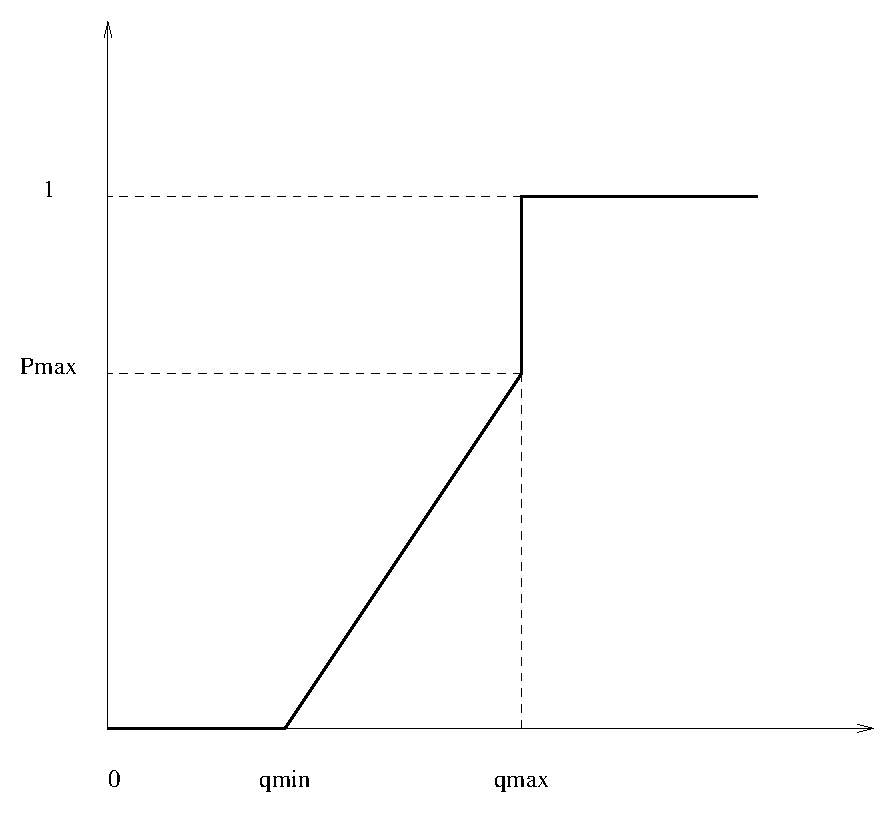
\includegraphics[width=0.8\linewidth]{figures/RED.eps}
\caption{Dropping probability as a function of average queue delay in RED.}
\label{fig:RED}
\end{figure}
  
It is straightforward to generalize RED to weighted RED in which different packets use different profiles (different configuration parameters) in order to prioritize some packets over the others.
Typically, packets with higher dropping precedence are exposed to more aggressive RED profiles.

\section{Explicit Congestion Notification}

It is sad to drop packets when they are half-way towards their destination, but in principle it is the only mechanism to signal TCP that it has to reduce its sending rate.
There is an alternative, introduced in  RFC 3168 \cite{rfc3168} which allows notifying TCP without dropping packets.

First it is necessary that both communication endpoints can support ECN and agree to use it.
If they do, they will use the least two significant bits of the DiffServ field to indicate it.
These bits will be set to either 10 or 01 if ECN is being used, and 00 otherwise.

If a router that supports ECN decides to drop a packet, it will first check whether the packet belongs to a flow that supports ECN.
If it does, it will set the ECN bits of the packet to 11 and will not drop the packet.
The receiving host will use the Explicit Congestion Echo (ECE) flag to notify the sender.
The sender will reduce the congestion window and activate the Congestion Window Reduced (CWR) flag.
The receiver will keep ECE activated in all the transmitted packets until receives the CWR from the sender.

Upon reception of this ECE, the originating host will reduce its congestion window (and thus its transmitting rate) just as if a packet dropped has occurred.
The advantages are that there is no need for packet re-transmission and that the reaction time is shorter.
This way, it is possible to achieve congestion control without packet dropping.

A particularly noticeable improvement is perceived in interactive protocols such as HTTP, telnet and SMPTP.
If the last packet (and probably single) packet of a message is dropped, the RTO expires and a retransmission occurs.
This retransmission can be avoided using ECN.

Despite all the advantages of ECN, it is not widely used yet.
The reasons are that, for being effective, it is necessary that both endpoints and also the network equipment supports ECN.
Furthermore, there are broken implementations in networking devices that do not recognize ECN and simply drop the packets that include 10 or 01 in the ECN field.

\section{CoDel}
The latest trend in AQM is Controlled Delay (or CoDel) \cite{nichols2012cqd}, which discards packets when the minimum queue occupation exceeds a threshold (in time).
This technique seem to be easier to configure and provide better link utilization while preventing bufferbloat.
